\subsubsection{Что такое "токовое зеркало?" Где оно находит применение?}

Усилительные каскады с управляемыми источниками тока применяются в интегральной схемотехнике.

Управляемые источники тока представляют собой либо цепи, питающие нагрузку определенным током, либо цепи, отбирающие этот ток от нагрузки. Из-за технологических особенностей вторая группа цепей получила большее распространение. 

Упрощенная схема управляемого источника:
\begin{center}
	\begin{figure}[h!]
		\center{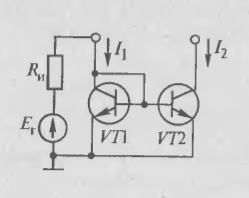
\includegraphics[scale=0.7]{Imirr.png}}
		\caption{}	
	\end{figure}
\end{center}
В этой схеме транзистор VT1 охвачен 100$\%$ обратной связью. Ток, протекающий в цепи базы,приблизительно в B раз меньше тока в цепи коллектора. При этом, если транзистор VT2, эмиттерный переход которого подключен параллельно эмиттерному переходу транзистора VT1, имеет полностью идентичные характеристики с транзистором VT1, то в цепи его базы протекает ток $I_{b_1} = I_{b_2}$. Соответственно равны и коллекторные токи. Общий входной ток каскада $I_1$ складывается из двух базовых токов и коллекторного тока транзистора VT1. Ток $I_2$ считается выходным. Тогда отношение входного и выходного токов можно записать как 
$$
\frac{I_2}{I_1} = \frac{I_{K1}}{I_{K1} + 2(I_{K1}/B)} \approx 1
$$

Нетрудно увидеть, что при использовании идентичных транзисторов с большим коэффициентом передачи базового тока B, выходной ток практически равен входному. Поэтому подобные управляемые источники тока называют отражателями тока или \textbf{токовыми зеркалами}

Таким образом, токовое зеркало — генератор тока, управляемый током. Чаще всего выходной ток равен управляющему или отличается от него в целое число раз.

Их нередко применяют в дифференциальных усилителях:
\begin{center}
	\begin{figure}[h!]
		\center{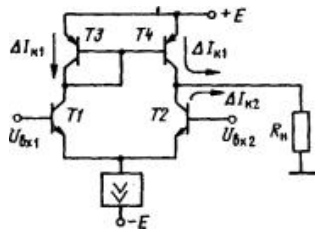
\includegraphics[scale=0.7]{DMirr.png}}
		\caption{}	
	\end{figure}
\end{center}


Работа токового зеркала «программируется» путём задания коллекторного тока транзистора VT1. Фактически, ГСТ и задает. (коллекторный ток VT2 поведёт себя так же ввиду симметрии схемы) Напряжение $U_{be}$ для VT1 устанавливается в соответствии с заданным током, температурой окружающей среды и типом транзистора. В результате оказывается заданным режим схемы. Небольшими базовыми токами можно пренебречь.

Рассмот­рим схему ДУ с токовым зеркалом. Транзисторы VТ1 и VТ2 выполняют свои обычные функции усилительных элементов, а транзисторы VТЗ и VТ4 — нагрузочных элементов, т. е. резисторов. Транзистор VТЗ включен по схеме диода. Предположим, что на базу у транзистора VТ1 приложена в рассматриваемый момент положительная полуволна $\Delta U_{in}$. В результате в цепи транзистора VТЗ возникает приращение тока $\Delta I_{K1}$ протекающего в направлении, указанном стрелкой. На эту дельту должно ответить приращение напряжения между эмиттером и базой транзистора VT3. Если возникло для VT3 => возникло и для VT4. Таким образом в цепи эмиттер—коллектор VТ4 возникает приращение тока, практически равное $\Delta I_{K1}$, поскольку в ДУ плечи симметричны. Пусть тогда же на базу транзистора VТ2 приложена отрицательная полуволна $\Delta U_{in}$. Следовательно, в цепи его коллектора появилось отрицательное приращение тока $\Delta I_{K2}$  протекающего в направлении, указанном стрелкой. При этом приращение тока нагрузки для ДУ равно $\Delta I_{K1} + \Delta I_{K2}$, 

В данном случае
$$
Кuдиф = \beta R_{out}/(R_{inTR_{oe}}).
$$  

Выше, чем у дифкаскада на резисторах. Выгодно увеличивать $R_{out}$, поэтому часто нагрузку через усилительные каскады на БП.(ОЭ).

Необходимо также отметить, что для рассматриваемого варианта ДУ в режиме покоя ток нагрузки равен нулю.
